This chapter details the complete methodological framework used for developing, training, and evaluating deep learning models for gait-based individual identification using Wi-Fi Channel State Information (CSI). The methodology encompasses data preprocessing, sliding-window sequence preparation, dual-stream feature extraction, model architecture design, MLOps-driven experimentation, and evaluation protocols. To enhance clarity, this chapter integrates system architecture diagrams and model-specific computational flows.

\section{Overall System Architecture}

Figure~\ref{fig:system_architecture} shows the high-level architecture of the proposed CSI-based identification pipeline.

\begin{figure}[htbp]
\centering
\resizebox{\textwidth}{!}{%
\begin{tikzpicture}[
    node distance=2.6cm and 2cm,
    box/.style={
        draw,
        rounded corners,
        align=center,
        minimum width=3.5cm,
        minimum height=1.1cm
    }
]

% ---------- ROW 1 ----------
\node[box, fill=blue!15] (data)
    {Raw CSI \\ CSV Files};

\node[box, fill=green!15, right=of data] (preprocess)
    {Preprocessing \\ \scriptsize (Parsing, Scaling, Windowing)};

\node[box, fill=yellow!20, right=of preprocess] (feature)
    {CSI + Metadata \\ Feature Streams};

% ---------- ROW 2 ----------
\node[box, fill=orange!20, below=1.8cm of feature] (models)
    {Deep Learning Models \\ \scriptsize CSILSTMNet, DenseNet1D,\\ EfficientNet1D-LSTM, MobileNetV3-1D-LSTM};

\node[box, fill=red!20, left=of models] (classifier)
    {Softmax \\ Classifier};

\node[box, fill=purple!20, left=of classifier] (output)
    {Predicted \\ Subject ID};

% ---------- ARROWS ----------
\draw[->, thick] (data) -- (preprocess);
\draw[->, thick] (preprocess) -- (feature);
\draw[->, thick] (feature) -- (models);
\draw[->, thick] (models) -- (classifier);
\draw[->, thick] (classifier) -- (output);

\end{tikzpicture}
} % end resizebox
\caption{System architecture for CSI-based gait identification.}
\label{fig:system_architecture}
\end{figure}

As shown in Figure~\ref{fig:wifi_csi_pipeline_1}, the pipeline begins by loading configurations and preparing the dataset...


\begin{figure}[H]
\centering
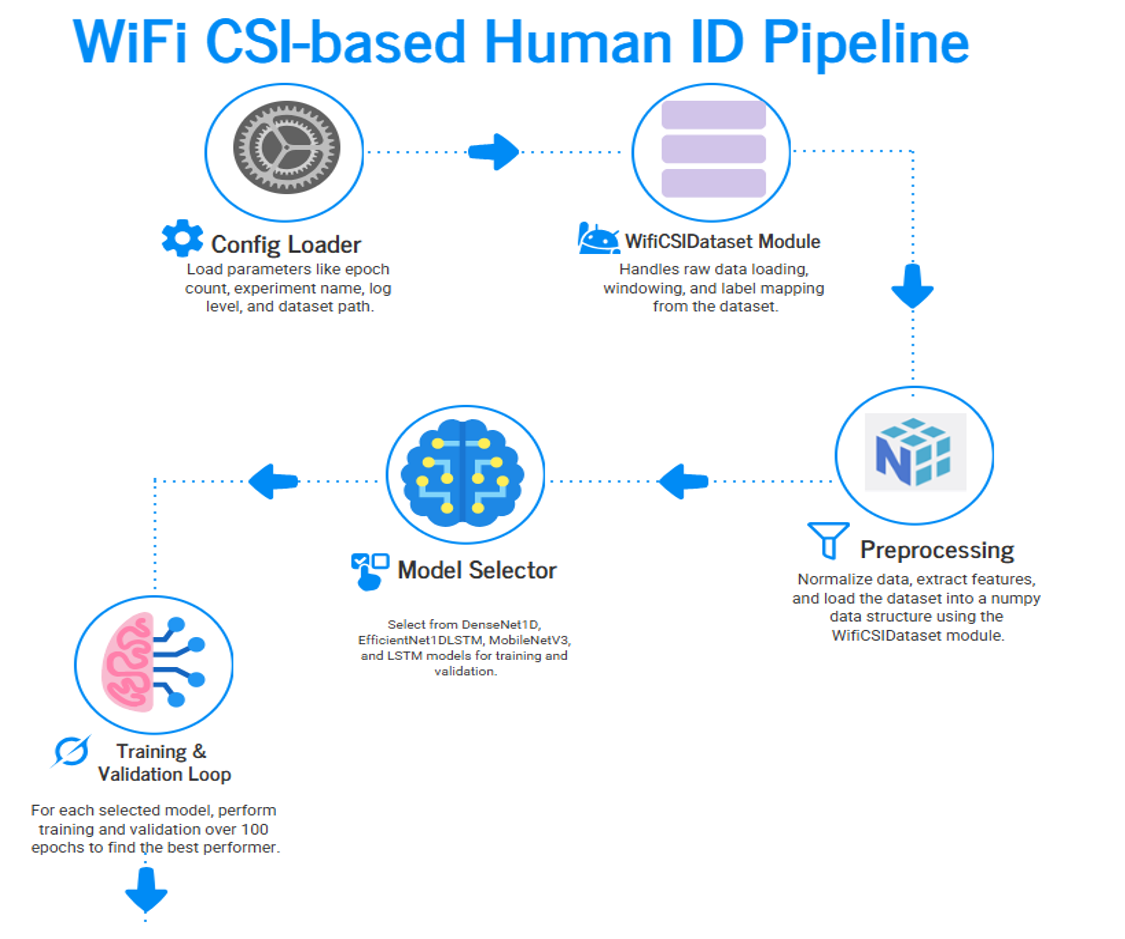
\includegraphics[width=\textwidth]{figures/pipeline_diagram_1.png}
\caption{Overall WiFi CSI-based Human Identification Pipeline.  
This diagram illustrates the high-level flow of configuration loading, dataset handling, preprocessing, model selection, and the training-validation loop used in this research.}
\label{fig:wifi_csi_pipeline_1}
\end{figure}

Figure~\ref{fig:wifi_csi_pipeline_2} further illustrates the internal training and validation loop...

\begin{figure}[H]
\centering
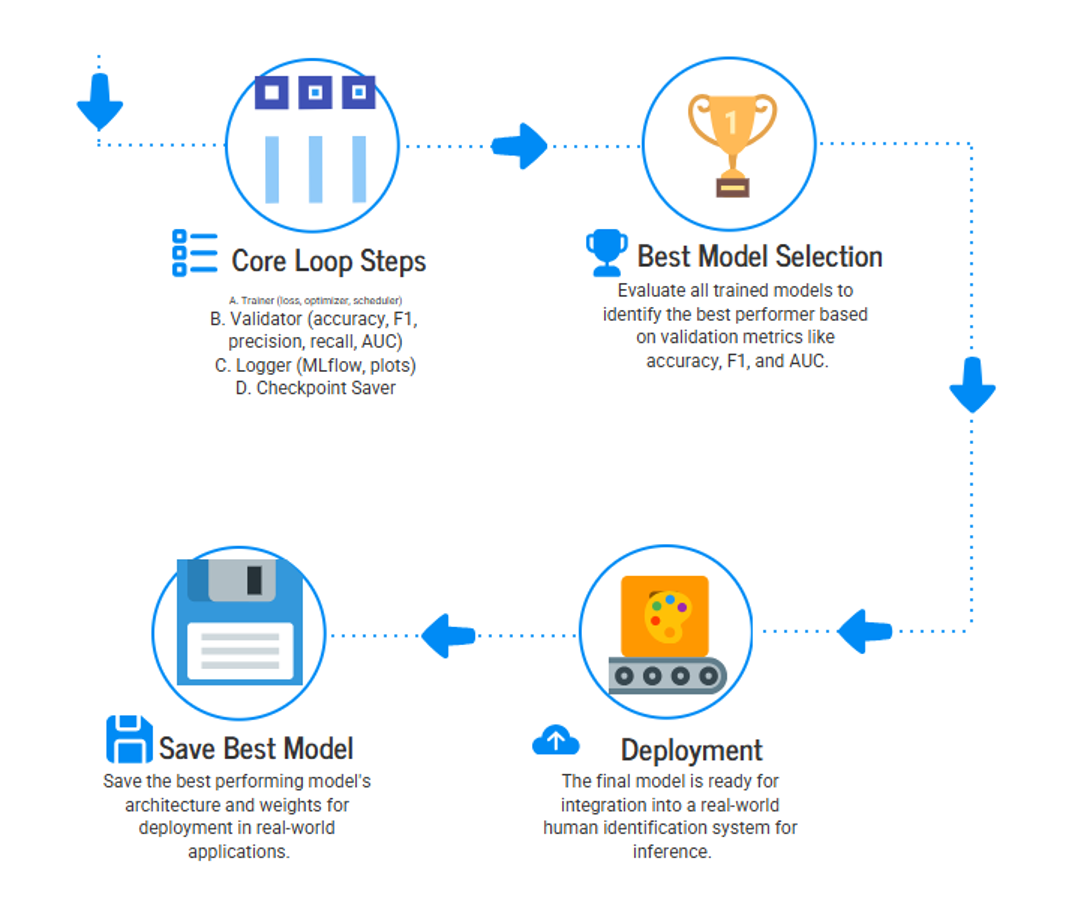
\includegraphics[width=\textwidth]{figures/pipeline_diagram_2.png}
\caption{Detailed Training and Model Selection Workflow.  
This slide illustrates the dataset preprocessing, model selection across four architectures, and the training–validation loop executed for every experiment using the MLOps-enabled pipeline.}
\label{fig:wifi_csi_pipeline_2}
\end{figure}


\section{CSI Data and Preprocessing Pipeline}
\label{sec:preprocessing}

The raw Wi-Fi Channel State Information (CSI) recordings contain both metadata and complex-valued CSI measurements captured across 3 X 30 OFDM subcarriers. Before the signals can be used for model training, they must be transformed into a stable, real-valued representation and organized into fixed-length temporal windows suitable for deep learning. The preprocessing pipeline used in this study follows the conceptual flow illustrated earlier (Fig.~\ref{fig:wifi_csi_pipeline_1}) and consists of two major stages: complex CSI decoding and feature construction.

\subsection{Complex CSI Interpretation}

Each CSI measurement is a complex number describing the amplitude and phase response of an individual subcarrier:
\[
h_i(t) = a_i(t)e^{j\phi_i(t)} = \mathrm{Re}(h_i(t)) + j\,\mathrm{Im}(h_i(t)),
\]
where \(a_i(t)\) denotes the signal amplitude, \(\phi_i(t)\) represents the phase shift caused by multipath propagation and human movement, \(i\) is the subcarrier index, and \(t\) is the temporal index.

Following standard practice in Wi-Fi sensing, the complex CSI values are converted into a real-valued representation using amplitude extraction:
\[
|h_i(t)| = \sqrt{\left(\mathrm{Re}(h_i(t))\right)^2 + \left(\mathrm{Im}(h_i(t))\right)^2}.
\]
This step ensures numerical stability and removes phase discontinuities that arise from hardware imperfections. The conversion is implemented during parsing, as shown in the highlighted code fragment in Fig.~\ref{fig:absolute value}, where each CSI row is reconstructed from its complex form.

\begin{figure}[H]
    \centering
    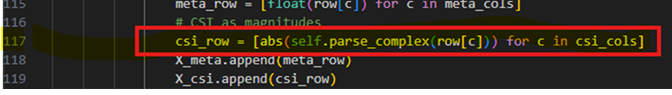
\includegraphics[width=0.7\textwidth]{figures/abs_value.png}
    \caption{Calculating absolute value of a Complex number representing WIFI CSI Data-point}
    \label{fig:absolute value}
\end{figure}
\subsection{Metadata Extraction}

The CSI files also embed a fixed set of transmit–receive metadata fields such as:
\begin{itemize}
    \item Received Signal Strength Indicator (RSSI),
    \item Automatic Gain Control (AGC) values,
    \item Packet-level timestamps,
    \item Antenna permutation indices,
    \item Transmitter and receiver identifiers.
\end{itemize}

These metadata features provide coarse-grained context about the wireless link and are processed in parallel with CSI amplitude values. All metadata fields are standardized using \texttt{StandardScaler} to ensure consistent scaling across batches.

\subsection{Sliding-Window Segmentation}

Since CSI streams are long, noisy, and strongly influenced by human motion dynamics, they are segmented into fixed-size windows. A sliding-window strategy with window length \(128\) and stride \(64\) is employed:
\begin{itemize}
    \item increases sample density,
    \item preserves temporal continuity,
    \item ensures coverage over complete gait cycles.
\end{itemize}

Each CSI window is therefore represented as:
\[
X_{\text{CSI}} \in \mathbb{R}^{128 \times 90},
\qquad
X_{\text{META}} \in \mathbb{R}^{128 \times 12},
\]
where the CSI tensor captures subcarrier-wise temporal evolution, and the metadata tensor encodes link-level temporal variation.

\subsection{Dual-Branch Input Construction}

The final preprocessed dataset consists of synchronized CSI and metadata sequences. These are consumed by dual-branch deep learning architectures, where:
\begin{itemize}
    \item the CSI branch (DenseNet1D, EfficientNet1D-LSTM, MobileNetV3-1D-LSTM) learns fine-grained spatial–temporal patterns from amplitude sequences,
    \item the metadata branch (LSTM-based) models link-level dynamics that complement CSI features.
\end{itemize}

This structured transformation—from complex CSI samples to windowed amplitude–metadata sequences—establishes a clean, robust input pipeline supporting accurate gait-based human identification models.


\section{Model Architectures}

\begin{table}[H]
\scriptsize
\centering
\caption{Models Used for Training: Overview}
\label{tab:Table4_1}

\begin{tabular}{
    | p{3.5cm}     % Model Name
    | p{3cm}     % CSI Core
    | p{3cm}     % Metadata Core
    | p{5cm}     % Key Features
|}
\hline
\textbf{Model Name} &
\textbf{CSI Processing Core} &
\textbf{Metadata Processing Core} &
\textbf{Key Features} \\
\hline

\textbf{CSILSTMNet} &
Standard LSTM &
Standard LSTM &
Uses two parallel LSTMs (one for CSI and one for metadata).  
The final hidden states are concatenated to form the joint representation used for classification. \\
\hline

\textbf{DenseNet1D} &
Dense Block 1D CNN &
Bidirectional LSTM &
Uses 1D CNN blocks (DenseBlock1D) followed by global pooling for CSI, combined with a Bi-LSTM for metadata.
\\
\hline


\textbf{EfficientNet1DLSTM} &
MBConv1D Blocks &
Bidirectional LSTM &
Leverages \textbf{Mobile Inverted Bottleneck (MBConv)} blocks (stem, mbconv1-3) designed for efficiency, combined with a Bi-LSTM.\\
\hline

\textbf{MobileNetV3\_1D\_LSTM} &
MobileNetV3 Block 1D &
Bidirectional LSTM &
Incorporates specialized blocks (including depthwise separable convolutions and Squeeze-and-Excitation (SE) layers) optimized for mobile/efficient computing, combined with a Bi-LSTM.\\
\hline

\end{tabular}

\end{table}



\subsection{CSILSTMNet}

 \begin{figure}[H]
\centering
\resizebox{\textwidth}{!}{%
\begin{tikzpicture}[node distance=1.5cm]
    \node (csi) [draw, rounded corners, fill=blue!10, minimum width=3cm] {CSI Sequence};
    \node (meta) [draw, rounded corners, fill=green!10, below=1cm of csi, minimum width=3cm] {Metadata Sequence};

    \node (csi_lstm) [draw, right=2.8cm of csi, fill=blue!20, rounded corners, minimum width=3cm]
    {LSTM$_{\text{CSI}}$};
    \node (meta_lstm) [draw, right=2.8cm of meta, fill=green!20, rounded corners, minimum width=3cm]
    {LSTM$_{\text{META}}$};

    \node (concat) [draw, right=2.8cm of csi_lstm, fill=yellow!20, rounded corners, minimum width=3cm]
    {Concatenate};

    \node (fc) [draw, right=2.8cm of concat, fill=red!20, rounded corners, minimum width=3cm]
    {Fully Connected};

    \draw[->] (csi) -- (csi_lstm);
    \draw[->] (meta) -- (meta_lstm);
    \draw[->] (csi_lstm) -- (concat);
    \draw[->] (meta_lstm) -- (concat);
    \draw[->] (concat) -- (fc);
\end{tikzpicture}
} % END resizebox
\caption{CSILSTMNet architecture.}
\end{figure}


A dual-LSTM structure extracts temporal features independently from CSI and metadata, which are later fused.

\subsection{DenseNet1D Architecture Diagram}

\begin{figure}[H]
\centering
\resizebox{\textwidth}{!}{%
\begin{tikzpicture}[
    node distance=2.2cm and 1.6cm,
    box/.style={
        draw,
        rounded corners,
        minimum width=3.3cm,
        minimum height=1cm,
        align=center
    }
]

% ========== ROW 1 (left → right) ==========
\node[box, fill=blue!10] (input) {CSI Sequence};

\node[box, fill=orange!20, right=of input] (conv)
    {Initial 1D Conv};

\node[box, fill=orange!30, right=of conv] (dense)
    {Dense Block};

% ========== ROW 2 (wrap downward, right → left) ==========
\node[box, fill=yellow!20, below=of dense] (transition)
    {Transition Layer};

\node[box, fill=green!20, left=of transition] (lstm)
    {LSTM$_{\text{META}}$};

\node[box, fill=red!20, left=of lstm] (fc)
    {Classifier};

% ========== ARROWS ==========
% Top row arrows
\draw[->, thick] (input) -- (conv);
\draw[->, thick] (conv) -- (dense);

% Down arrow
\draw[->, thick] (dense) -- (transition);

% Bottom row arrows (right → left)
\draw[->, thick] (transition) -- (lstm);
\draw[->, thick] (lstm) -- (fc);

\end{tikzpicture}
}
\caption{DenseNet1D architecture.}
\label{fig:densenet_arch}
\end{figure}




\subsection{EfficientNet1D-LSTM Diagram}

\begin{figure}[H]
\centering
\resizebox{\textwidth}{!}{%
\begin{tikzpicture}[
    node distance=2.2cm and 1.6cm,
    box/.style={
        draw,
        rounded corners,
        minimum width=3.3cm,
        minimum height=1cm,
        align=center
    }
]

% ===== ROW 1: CSI feature extractor (left → right) =====
\node[box, fill=blue!10] (in) {CSI Input};

\node[box, fill=green!15, right=of in] (stem) {Stem Conv};

\node[box, fill=yellow!20, right=of stem] (mb1) {MBConv Block 1};

\node[box, fill=yellow!30, right=of mb1] (mb2) {MBConv Block 2};

\node[box, fill=yellow!40, right=of mb2] (mb3) {MBConv Block 3};

% ===== ROW 2: pooling + metadata + classifier =====
\node[box, fill=purple!20, below=of mb3] (pool) {Global Pool};

\node[box, fill=red!20, left=of pool] (fc) {Fully Connected};

\node[box, fill=orange!20, below=of mb1] (meta_lstm) {Metadata LSTM};

% ===== ARROWS =====
% top row
\draw[->, thick] (in) -- (stem);
\draw[->, thick] (stem) -- (mb1);
\draw[->, thick] (mb1) -- (mb2);
\draw[->, thick] (mb2) -- (mb3);

% down to row 2
\draw[->, thick] (mb3) -- (pool);

% row 2 + fusion
\draw[->, thick] (pool) -- (fc);
\draw[->, thick] (meta_lstm) -- (fc);

\end{tikzpicture}
}%
\caption{EfficientNet1DLSTM architecture.}
\label{fig:efficientnet1d_lstm_arch}
\end{figure}


\subsection{MobileNetV3-1D-LSTM Diagram}

 \begin{figure}[H]
\centering
\resizebox{\textwidth}{!}{%
\begin{tikzpicture}[
    node distance=2.2cm and 1.6cm,
    box/.style={
        draw,
        rounded corners,
        minimum width=3.3cm,
        minimum height=1cm,
        align=center
    }
]

% ===== TOP ROW =====
\node[box, fill=blue!10] (csi) {CSI Input};

\node[box, fill=orange!20, right=of csi] (mb1)
    {MobileNetV3 \\ Block 1};

\node[box, fill=orange!30, right=of mb1] (mb2)
    {MobileNetV3 \\ Block 2};

\node[box, fill=purple!15, right=of mb2] (pool)
    {Global Pool};

% ===== BOTTOM ROW =====
\node[box, fill=green!20, below=of mb2] (meta)
    {Metadata LSTM};

\node[box, fill=red!20, right=of meta] (fc)
    {Fully Connected};

% ===== ARROWS TOP ROW =====
\draw[->, thick] (csi) -- (mb1);
\draw[->, thick] (mb1) -- (mb2);
\draw[->, thick] (mb2) -- (pool);

% ===== CONNECTION BETWEEN ROWS =====
\draw[->, thick] (pool.south) -- ++(0,-1.0) -| (fc.north);

% ===== BOTTOM ROW ARROW =====
\draw[->, thick] (meta) -- (fc);

\end{tikzpicture}
}
\caption{MobileNetV3-1D-LSTM architecture.}
\label{fig:mobilenetv3_1d_lstm_arch}
\end{figure}




\section{Training Process}

The training pipeline includes:
\begin{itemize}
    \item Adam/AdamW optimizers
    \item Label smoothing
    \item Gradient clipping
    \item Batch-wise normalization
\end{itemize}

Each model is trained for 100 epochs with early stopping patience of 15 epochs.

\section{MLflow-Based MLOps Integration}
\label{sec:mlops}

To ensure systematic experimentation, reproducibility, and transparent model comparison, the entire training pipeline was integrated with MLflow. This MLOps framework provided seamless logging of all experiments conducted across the four architectures—DenseNet1D, EfficientNet1D-LSTM, MobileNetV3\_1D\_LSTM, and CSILSTMNet.

\subsection{Experiment Tracking and Automated Logging}

MLflow automatically recorded every training run, capturing:
\begin{itemize}
    \item \textbf{Hyperparameters:} learning rate, batch size, weight decay, optimizer configuration.
    \item \textbf{Training dynamics:} epoch-wise accuracy, F1-score, precision, recall, AUC, and loss curves.
    \item \textbf{Model artifacts:} saved checkpoints, confusion matrices, and evaluation reports.
    \item \textbf{Model signatures:} input--output schema for consistent deployment.
    \item \textbf{Version control:} automatic assignment of run IDs and model version tagging.
\end{itemize}

\subsection{Why MLflow Integration Matters}

The integration enabled:
\begin{itemize}
    \item \textbf{Side-by-side model comparison} through MLflow dashboards, supporting direct evaluation of accuracy, convergence behaviour, and generalization performance.
    \item \textbf{Reproducibility} of all experiments, ensuring that results can be revalidated or extended without ambiguity.
    \item \textbf{Transparent performance tracking}, allowing systematic identification of the best-performing model across 100+ epochs.
    \item \textbf{Data-driven model selection}, based on objective metrics rather than manually inspected logs.
\end{itemize}
\begin{figure}[htbp]
\centering

% ---------- Row 1: Training metrics ----------
\begin{subfigure}{0.32\textwidth}
    \centering
    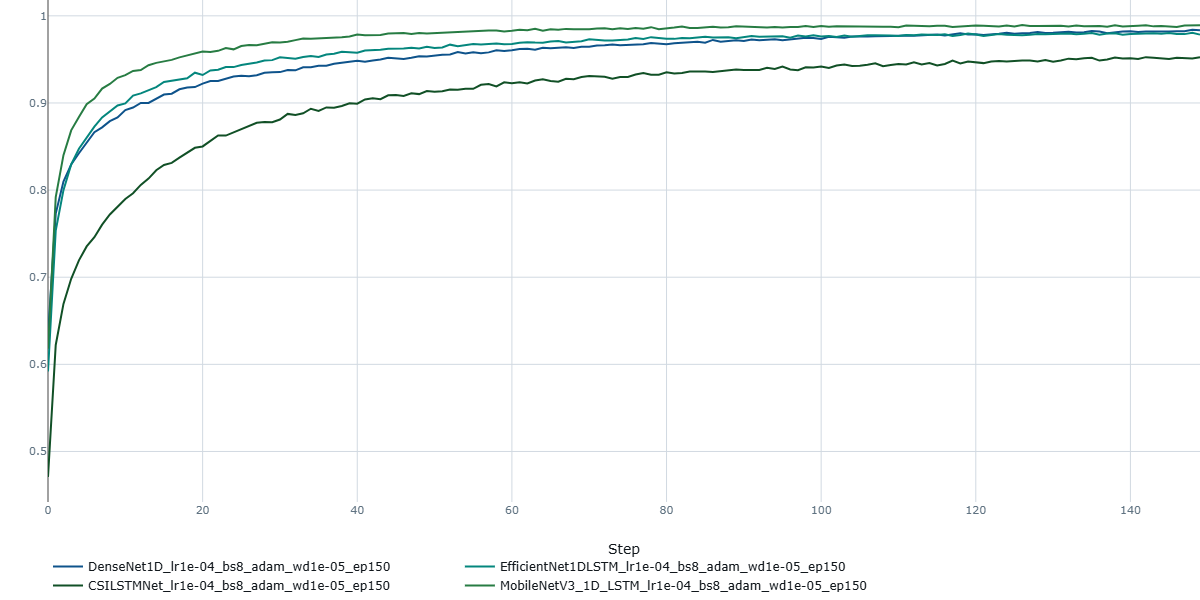
\includegraphics[width=\linewidth]{figures/mlops/Training Accuracy Curve.png}
    \caption{Training accuracy}
    \label{fig:mlflow_train_acc}
\end{subfigure}
\hfill
\begin{subfigure}{0.32\textwidth}
    \centering
    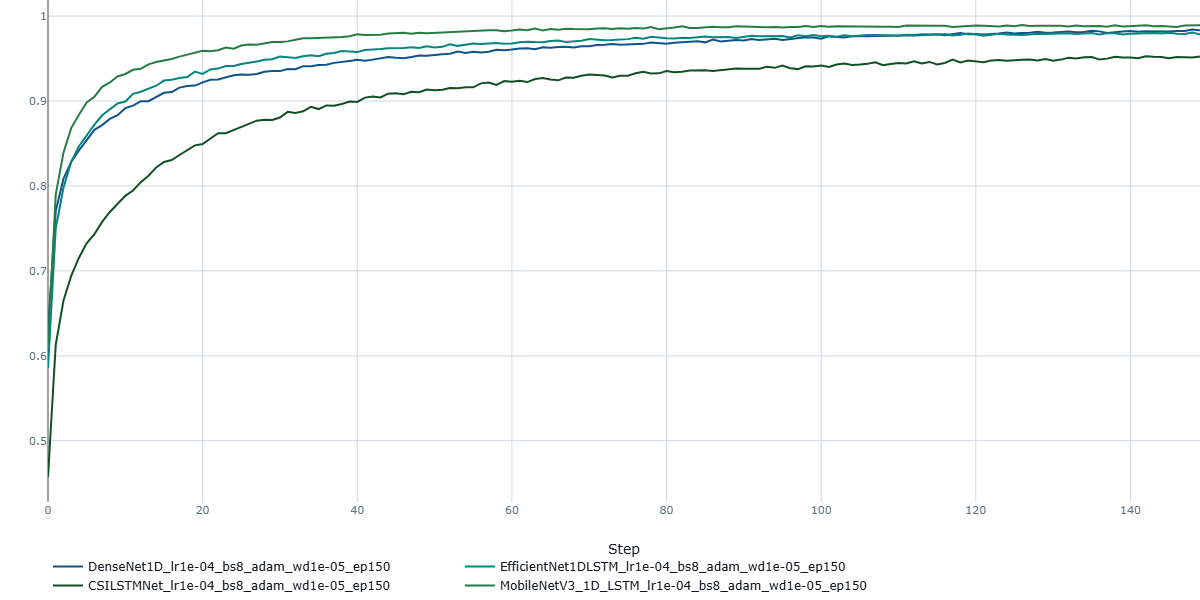
\includegraphics[width=\linewidth]{figures/mlops/Training Precision Curve.png}
    \caption{Training precision}
    \label{fig:mlflow_train_prec}
\end{subfigure}
\hfill
\begin{subfigure}{0.32\textwidth}
    \centering
    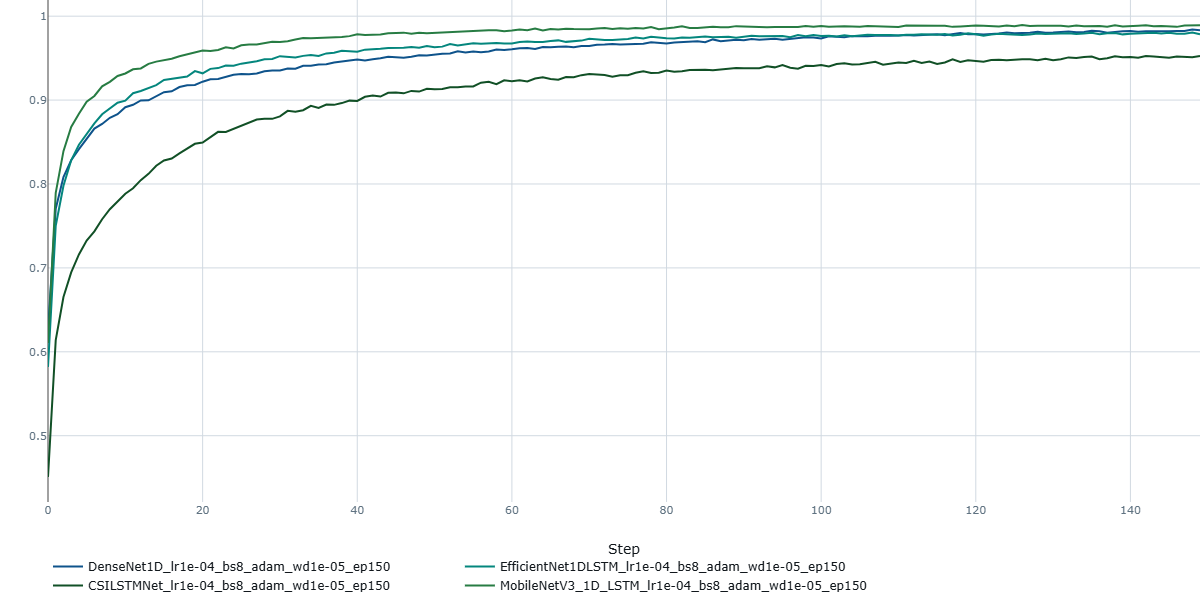
\includegraphics[width=\linewidth]{figures/mlops/Training F1 Score.png}
    \caption{Training F1-score}
    \label{fig:mlflow_train_f1}
\end{subfigure}

\vspace{0.6em}

% ---------- Row 2: Validation metrics ----------
\begin{subfigure}{0.32\textwidth}
    \centering
    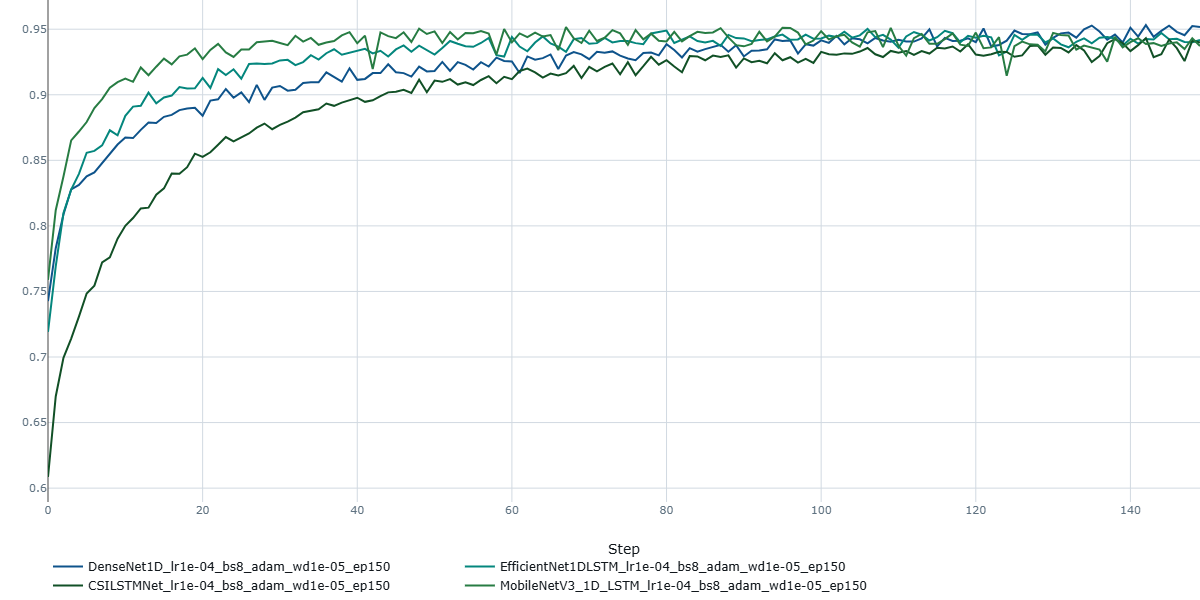
\includegraphics[width=\linewidth]{figures/mlops/Validation Accuracy Curve.png}
    \caption{Validation accuracy}
    \label{fig:mlflow_val_acc}
\end{subfigure}
\hfill
\begin{subfigure}{0.32\textwidth}
    \centering
    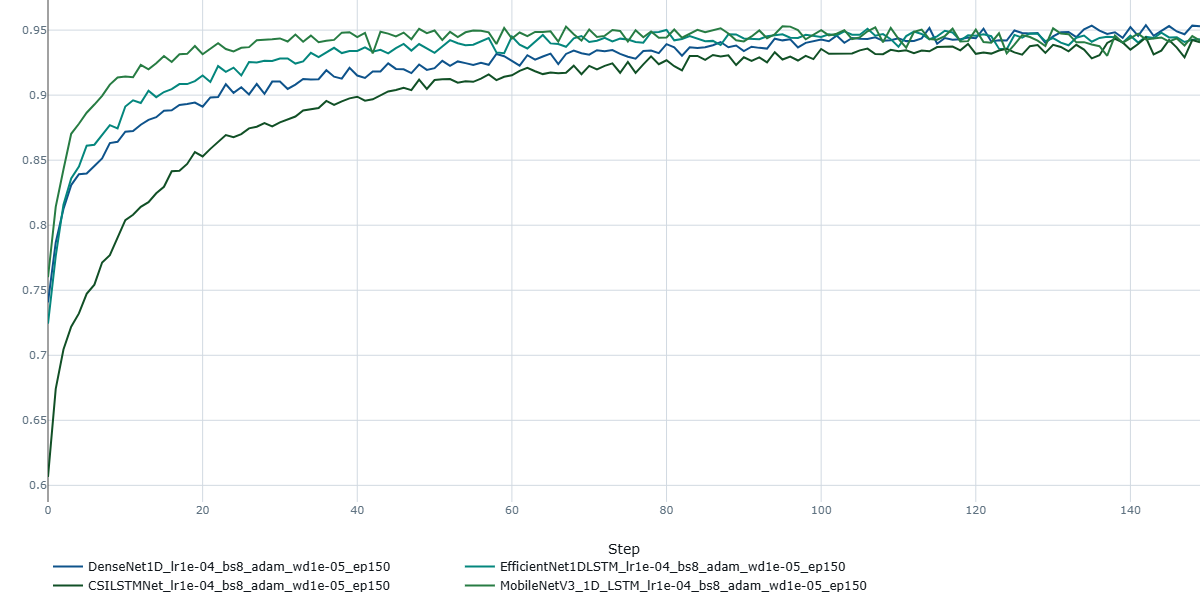
\includegraphics[width=\linewidth]{figures/mlops/Validation Precision Curve.png}
    \caption{Validation precision}
    \label{fig:mlflow_val_prec}
\end{subfigure}
\hfill
\begin{subfigure}{0.32\textwidth}
    \centering
    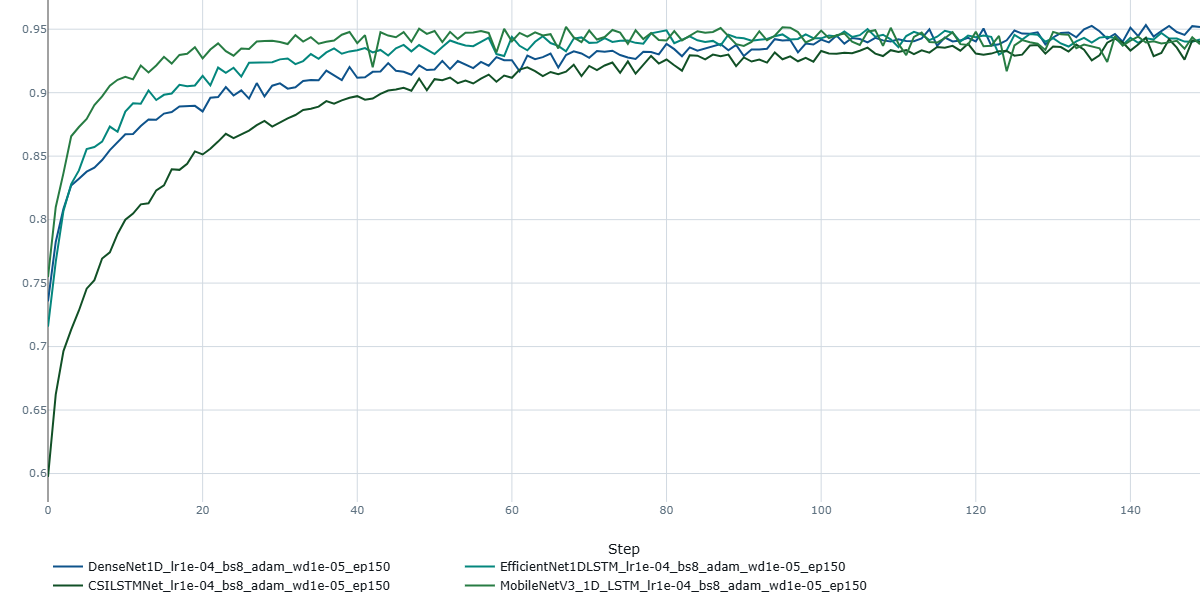
\includegraphics[width=\linewidth]{figures/mlops/Validation F1 Score.png}
    \caption{Validation F1-score}
    \label{fig:mlflow_val_f1}
\end{subfigure}

\vspace{0.6em}

% ---------- Row 3: Loss curves ----------
\begin{subfigure}{0.32\textwidth}
    \centering
    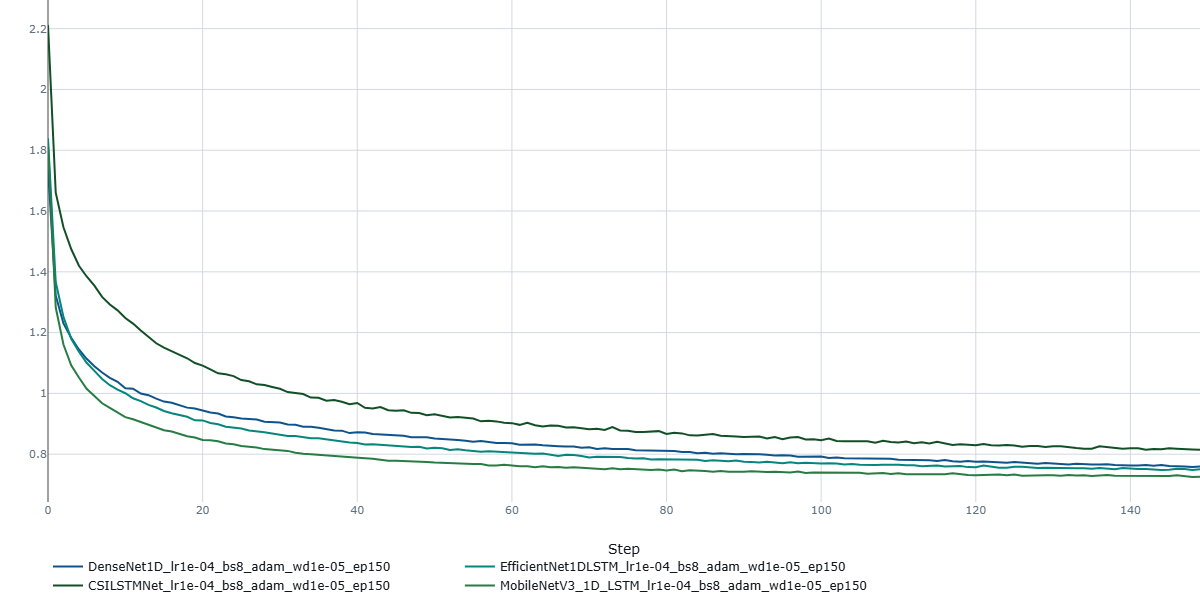
\includegraphics[width=\linewidth]{figures/mlops/Training Loss Curve.png}
    \caption{Training loss}
    \label{fig:mlflow_train_loss}
\end{subfigure}
\hfill
\begin{subfigure}{0.32\textwidth}
    \centering
    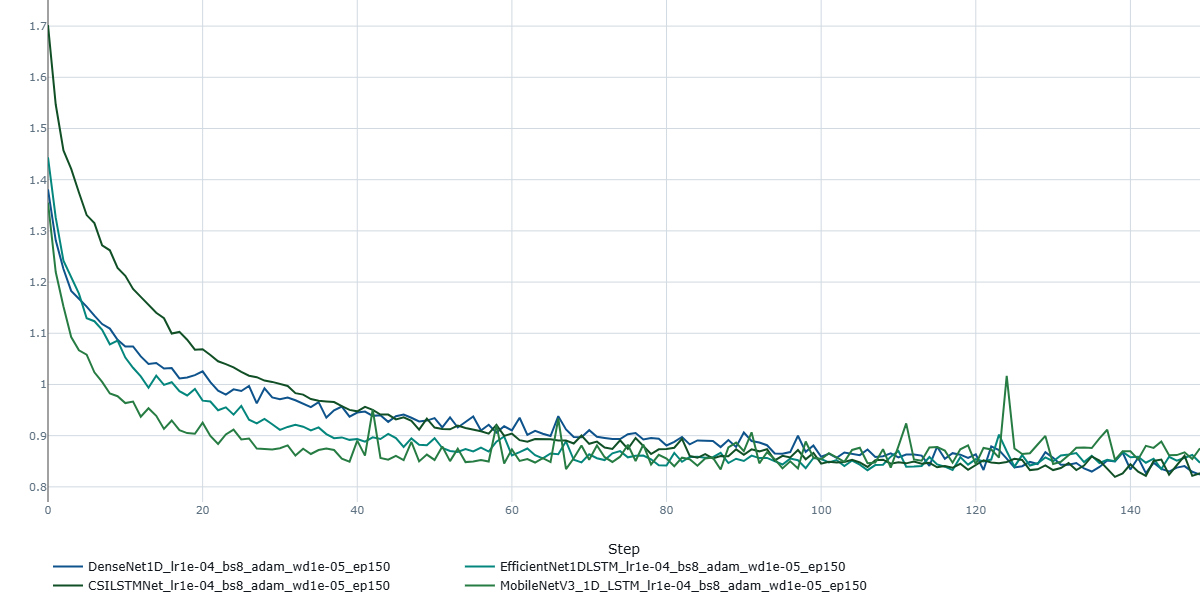
\includegraphics[width=\linewidth]{figures/mlops/Validation Loss Curve.png}
    \caption{Validation loss}
    \label{fig:mlflow_val_loss}
\end{subfigure}

\caption{MLflow-based comparison of the four CSI models across training and validation accuracy, precision, F1-score, and loss curves over 150 epochs. These metrics were automatically logged by MLflow, enabling seamless model comparison and reproducible performance tracking.}
\label{fig:mlflow_metrics_overview}
\end{figure}

\subsection{Outcome}

By embedding MLflow into the workflow, this study gained structured experiment management, rich visual analytics, and reliable comparison across all architectures. The resulting insights directly informed hyperparameter optimization and reinforced the selection of DenseNet1D as the most accurate and stable model for Wi-Fi CSI–based identification.


\section{Evaluation Metrics}

The following metrics are computed:
\begin{itemize}
    \item Accuracy
    \item Precision, Recall, F1-score
    \item Confusion matrix
    \item Per-class identification accuracy
\end{itemize}

